% Agents 101: a gentle opening for a general software audience with no agent-building background.
% Sits ahead of langgraph_intro in the LangGraph seminar. Comment out the \input line there to switch off.

%%%%%%%%%%%%%%%%%%%%%%%%%%%%%%%%%%%%%%%%%%%%%%%%%%%%%%%%%%%%%%%%%%%%%%%%%%%%%%%%
% [Optional cut 2026-10-19 | LangGraph trim, move to the advanced part | restore by uncommenting this block]
% \begin{frame}[fragile]\frametitle{}
% \begin{center}
% {\Large Why Learn to Build Agents?}
% 
% \medskip
% {\small (Agents 101, before we touch LangGraph)}
% \end{center}
% \end{frame}

%%%%%%%%%%%%%%%%%%%%%%%%%%%%%%%%%%%%%%%%%%%%%%%%%%%
% [Optional cut 2026-10-19 | LangGraph trim, move to the advanced part | restore by uncommenting this block]
% \begin{frame}[fragile]\frametitle{From Answering to Doing}
% \begin{itemize}
% \item A chatbot \textbf{answers}: ``Here is how you could book a flight.''
% \item An agent \textbf{acts}: it searches, compares, books, and tells you when it is done.
% \item The difference is not a bigger model. It is a model \emph{plus tools plus a loop}.
% \item Anything you do by hand in several steps, across several tools, is a candidate for an agent.
% \end{itemize}
% \end{frame}

%%%%%%%%%%%%%%%%%%%%%%%%%%%%%%%%%%%%%%%%%%%%%%%%%%%
% [Optional cut 2026-10-19 | LangGraph trim, move to the advanced part | restore by uncommenting this block]
% \begin{frame}[fragile]\frametitle{Why This Is a Skill Worth Having}
% \begin{itemize}
% \item \textbf{It extends what you already do:} agents call APIs, read databases and run code, so they build on ordinary software skills.
% \item \textbf{It is where LLM work is moving:} from single prompts to systems that finish tasks.
% \item \textbf{It is a new kind of engineering:} you design behaviour, limits and checks, not only functions.
% \item \textbf{It is learnable:} the core idea has three parts: a brain, hands and a loop.
% \end{itemize}
% \end{frame}

%%%%%%%%%%%%%%%%%%%%%%%%%%%%%%%%%%%%%%%%%%%%%%%%%%%
\begin{frame}[fragile]\frametitle{Anatomy of an Agent: Brain, Hands, Loop}
\begin{center}
% [upgrade-deck: replaced 2026-10-19 | Task 1e | the fixed-height resizebox ran off the column in the 3-column CheatSheet; original: \resizebox{!}{0.55\textheight}{%]
\adjustbox{max width=\linewidth, max totalheight=0.55\textheight}{%
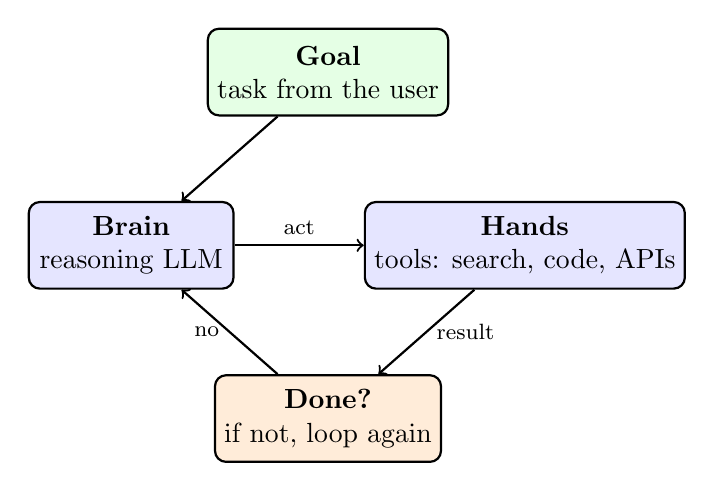
\begin{tikzpicture}[box/.style={draw, rounded corners, thick, minimum width=2.6cm, minimum height=1.1cm, align=center, fill=blue!10}]
\node[box] (brain) at (0,0) {\textbf{Brain}\\reasoning LLM};
\node[box] (tools) at (5,0) {\textbf{Hands}\\tools: search, code, APIs};
\node[box, fill=green!10] (goal) at (2.5,2.2) {\textbf{Goal}\\task from the user};
\node[box, fill=orange!15] (done) at (2.5,-2.2) {\textbf{Done?}\\if not, loop again};
\draw[->, thick] (goal) -- (brain);
\draw[->, thick] (brain) -- node[above] {\footnotesize act} (tools);
\draw[->, thick] (tools) -- node[right] {\footnotesize result} (done);
\draw[->, thick] (done) -- node[left] {\footnotesize no} (brain);
\end{tikzpicture}}
\end{center}
\begin{itemize}
% [upgrade-deck: commented out 2026-10-19 | Task 5c | three sentences split into three short points]
% \item The \textbf{brain} decides what to do next. The \textbf{hands} do it. The \textbf{loop} repeats until the task is complete.
\item The \textbf{brain} decides what to do next.
\item The \textbf{hands} do it.
\item The \textbf{loop} repeats until the task is complete.
\end{itemize}
\end{frame}

%%%%%%%%%%%%%%%%%%%%%%%%%%%%%%%%%%%%%%%%%%%%%%%%%%%
% [Optional cut 2026-10-19 | LangGraph trim, move to the advanced part | restore by uncommenting this block]
% \begin{frame}[fragile]\frametitle{One Loop, Step by Step}
% \begin{itemize}
% \item \textbf{Task:} ``Find the three newest open issues in our repo and email a summary to the team.''
% \item \textbf{Thought:} I need the list of issues first.
% \item \textbf{Action:} call the issue-tracker tool, sorted by date.
% \item \textbf{Observation:} three issue titles and links come back.
% \item \textbf{Thought:} now I can write the summary and send it.
% \item \textbf{Action:} call the email tool. \textbf{Observation:} sent. \textbf{Done.}
% \end{itemize}
% \end{frame}

%%%%%%%%%%%%%%%%%%%%%%%%%%%%%%%%%%%%%%%%%%%%%%%%%%%
% [Optional cut 2026-10-19 | LangGraph trim, move to the advanced part | restore by uncommenting this block]
% \begin{frame}[fragile]\frametitle{Sub-Agents: A Team Instead of a Soloist}
% \begin{itemize}
% \item One agent with too many tools and too long a task gets confused.
% \item Split the work: a \textbf{manager} agent hands pieces to \textbf{specialist} sub-agents.
% \item Each specialist has a narrow job, a short prompt and only the tools it needs.
% \item Same idea as a software team: one lead, a few focused engineers.
% \end{itemize}
% \end{frame}

%%%%%%%%%%%%%%%%%%%%%%%%%%%%%%%%%%%%%%%%%%%%%%%%%%%
% [Optional cut 2026-10-19 | LangGraph trim, move to the advanced part | restore by uncommenting this block]
% \begin{frame}[fragile]\frametitle{Agent Architectures at a Glance}
% \begin{center}
% \resizebox{\linewidth}{!}{%
% \begin{tabular}{lll}
% \toprule
% Architecture & Who decides the next step? & Trade-off \\
% \midrule
% Fixed workflow & The developer, always & Predictable, rigid \\
% Router & Developer's rules or one LLM choice & Simple branching, no loops \\
% Single agent (ReAct) & The LLM, every step & Flexible, can wander \\
% Graph or state machine & Developer draws the map, LLM picks the path & Controlled, flexible \\
% Multi-agent team & A manager LLM and specialists & Scales, harder to debug \\
% \bottomrule
% \end{tabular}}
% \end{center}
% \end{frame}

%%%%%%%%%%%%%%%%%%%%%%%%%%%%%%%%%%%%%%%%%%%%%%%%%%%
\begin{frame}[fragile]\frametitle{Where LangGraph Fits}
\begin{itemize}
\item LangGraph sits in the \textbf{semi-deterministic} middle: you draw the map, the LLM chooses the route.
\item You get loops, branches, memory and human approval points, with the path visible and testable.
\item That visibility is why teams use it when an agent must be reliable, not just clever.
\item The rest of this talk builds that map, one piece at a time.
\end{itemize}
\end{frame}

%%%%%%%%%%%%%%%%%%%%%%%%%%%%%%%%%%%%%%%%%%%%%%%%%%%
\begin{frame}[fragile]\frametitle{Quick Check: What Makes an Agent}
\begin{block}{Think About It}
Which system is an agent, in the sense used in this talk?
\begin{enumerate}
  \item[A.] A script that sends every customer email to an LLM for a one-line summary.
  \item[B.] An LLM that reads a request, picks a tool, checks the result and repeats until the task is done.
  \item[C.] A chatbot with a very large prompt and a friendly tone.
  \item[D.] A fixed pipeline of three LLM calls that always run in the same order.
\end{enumerate}
\end{block}
\end{frame}

%%%%%%%%%%%%%%%%%%%%%%%%%%%%%%%%%%%%%%%%%%%%%%%%%%%
\begin{frame}[fragile]\frametitle{Quick Check: What Makes an Agent}
\begin{block}{Answer}
\textbf{Correct: B.} An agent has a reasoning model, tools it can act with, and a loop that continues until
the task is complete. A (one fixed call), C (no tools, no loop) and D (a fixed order, with no decision
about the next step) lack at least one of the three parts.
\end{block}
\end{frame}
